\section{Основные понятия теории вероятностей}

\subsection{Элементы комбинаторики}
Для начала подружимся с комбинаторикой, взяв некоторую её проекцию на теорвер

\begin{to_thr}[]
    Пусть множества $A = \{a_1, \ldots, a_k\}$ состоит из $k$ элементов, а множество $B = \{b_1, \ldots, b_m\}$ -- из $m$ элементов. Тогда можно образовать равно $km$ пар $(a_i, b_j)$.
\end{to_thr}

\begin{to_thr}[]
    Общее количество различных наборов при выборе $k$ элементов из $n$ без возвращения и с учётом порядка равняется
    \begin{equation*}
        A_n^k = n \cdot (n-1) \cdot \ldots \cdot (n-k+1) = \frac{n!}{(n-k)!},
    \end{equation*}
    где $A_n^k$ называется \textit{числом размещений} из $n$ элементов по $k$ элементов. 
\end{to_thr}

\begin{to_thr}[]
    Общее количество различных наборов при выборе $k$ элементов из $n$ без возвращения и без учета порядка равняется
    \begin{equation*}
        C_n^k = \frac{A_n^k}{k!} = \frac{n!}{k! (n-k)!},
    \end{equation*}
    где число $C_n^k$ называется \textit{числом сочетаний} из $n$ элементов по $k$ элементов. 
\end{to_thr}

\green{
\begin{to_thr}[]
% вот тут не понял почему, но ладно
    Общее количество различных наборов при выборе $k$ элементов из $n$ с возвращением и без учёта порядка равняется
    \begin{equation*}
        C_{n+k-1}^k = C_{n+k-1}^{n-1}.
    \end{equation*}
\end{to_thr}
}

\subsection{События и операции над ними}
\begin{to_def}
    \textit{Пространством элементарных исходов} называют множество $\Omega$, содержащее все возможные взаимоисключающие результаты данного случайного эксперимента. Элементы множества $\Omega$ называются \textit{элементарными исходами} и обозначаются $\omega$.
\end{to_def}

\begin{to_def}
    \textit{Событиями} называются подмножества $\Omega$. Говорят, что \textit{произошло событие} $A$, если эксперимент завершился одним из элементарных исходов, входящих в множество $A$. 
\end{to_def}

Вообще в силу таких определений события и множества оказываются очень похожими, так что определены операции \textit{объединения}, \textit{пересечения}, \textit{дополнения}, а также взятия \textit{противоположеного} $\bar{A} = \Omega \backslash A$. Также можно выделить достоверное событие $\Omega$ и невозможное $\varnothing$. 

События $A$ и $B$ называются \textit{несовместными}, если они не могут произойти одновременно: $A \cap B = \varnothing$. События $A_1, \ldots, A_n$ называются \textit{попарно несовместными}, если несовместны любые два из них: $A_i \cap A_j = \varnothing, \ \forall i \neq j$. Говорят, что событие $A$ \textit{влечет} событие $B$ ($A \subseteq B$), если $A \Rightarrow B$. 



\subsection{Дискретное пространство элементарных исходов}
Пространство элементарных исходов назовём дискретным, если множество $\Omega$ конечно или счётно: $\Omega = \{\omega_1, .., \omega_n, \ldots\}$. 

\begin{to_def}
    Сопоставим каждому элементарному исходу $\omega_i$ число $p_i \in [0, 1]$ так, чтобы $\sum p_i = 1$. Вероятностью события $A$ называют число
    \begin{equation*}
        \P(A) = \sum_{\omega_i \in A} p_i,
    \end{equation*}
    где с случае $A = \varnothing$ считаем $\P(A) = 0$. 
\end{to_def}


\begin{to_def}[Классическое определение вероятности]
    Говорят, что эксперимент описывается \textit{классической вероятностной моделью}, если пространство его элементарных исходов состоит из конечного числа равновозможных исходов. Для любого события верно, что
    \begin{equation}
        \P (A) = \frac{\card A}{\card \Omega}.
    \end{equation}
    Эту формулу называют \textit{классическим определением вероятности}.
\end{to_def}

Тут стоит вспомнить три схемы из модели с урнами: 
схема выбора с возвращением и с учётом порядка ($n^k$), 
выбора без возвращения и с учётом порядка ($A_n^k$), а также выбора
без возвращения и без учёта порядка ($C_n^k$), 
описываются классической вероятностной моделью. 
А вот схема выбора с возвращением и без учёта порядкауже не описывается классической вероятностью. 


\subsubsection*{Пример с гипергеометрическим распределением}
 Из урны, в которой $K$ белых и $N - K$ чёрных шаров, наудачу и без возвращения вынимают $n$ шаров, где $n \leq N$.
Термин «наудачу» означает, что появление любого набора из $n$ шаров равновозможно. Найти вероятность того, что будет выбрано $k$ белых и $n - k$ чёрных шаров.

Результат -- набор из $n$ шаров. Общее число $\card \Omega = C_N^n$. Пусть $A_k$ -- событие, состоящее в том, что в наборе окажется $k$ белых и $n-k$ черных. Есть ровно $C_K^k$ способов выбрать $k$ белых шаров из $K$, и 
$C_{N-K}^{n-k}$ способов выбрать $n-k$ черных шаров из $N-K$. Тогда $\card A_k = C_K^k C_{N_K}^{n-k}$,
\begin{equation*}
    \P (A_k) = \frac{\card A_k}{\card \Omega} = \frac{C_K^k C_{N_K}^{n-k}}{C_N^n}.
\end{equation*}
Этот набор вероятностей называется \textit{гипергеометрическим распределением} вероятностей. 





\subsection{Дискретное пространство элементарных исходов}
Пространство элементарных исходов назовём дискретным, если множество $\Omega$ конечно или счётно: $\Omega = \{\omega_1, .., \omega_n, \ldots\}$. 

\begin{to_def}
    Сопоставим каждому элементарному исходу $\omega_i$ число $p_i \in [0, 1]$ так, чтобы $\sum p_i = 1$. Вероятностью события $A$ называют число
    \begin{equation*}
        \P(A) = \sum_{\omega_i \in A} p_i,
    \end{equation*}
    где с случае $A = \varnothing$ считаем $\P(A) = 0$. 
\end{to_def}


\begin{to_def}[Классическое определение вероятности]
    Говорят, что эксперимент описывается \textit{классической вероятностной моделью}, если пространство его элементарных исходов состоит из конечного числа равновозможных исходов. Для любого события верно, что
    \begin{equation}
        \P (A) = \frac{\card A}{\card \Omega}.
    \end{equation}
    Эту формулу называют \textit{классическим определением вероятности}.
\end{to_def}

Тут стоит вспомнить три схемы из модели с урнами: 
схема выбора с возвращением и с учётом порядка ($n^k$), 
выбора без возвращения и с учётом порядка ($A_n^k$), а также выбора
без возвращения и без учёта порядка ($C_n^k$), 
описываются классической вероятностной моделью. 
А вот схема выбора с возвращением и без учёта порядкауже не описывается классической вероятностью. 


\subsubsection*{Пример с гипергеометрическим распределением}
 Из урны, в которой $K$ белых и $N - K$ чёрных шаров, наудачу и без возвращения вынимают $n$ шаров, где $n \leq N$.
Термин «наудачу» означает, что появление любого набора из $n$ шаров равновозможно. Найти вероятность того, что будет выбрано $k$ белых и $n - k$ чёрных шаров.

Результат -- набор из $n$ шаров. Общее число $\card \Omega = C_N^n$. Пусть $A_k$ -- событие, состоящее в том, что в наборе окажется $k$ белых и $n-k$ черных. Есть ровно $C_K^k$ способов выбрать $k$ белых шаров из $K$, и 
$C_{N-K}^{n-k}$ способов выбрать $n-k$ черных шаров из $N-K$. Тогда $\card A_k = C_K^k C_{N_K}^{n-k}$,
\begin{equation*}
    \P (A_k) = \frac{\card A_k}{\card \Omega} = \frac{C_K^k C_{N_K}^{n-k}}{C_N^n}.
\end{equation*}
Этот набор вероятностей называется \textit{гипергеометрическим распределением} вероятностей. 





\subsection{Геометрическая вероятность}
\begin{to_def}
    Пусть некоторая область $\Omega \subset \mathbb{R}^k$ такая, что $\mu(\Omega)$ конечна. Пусть эксперимент состоит из равновероятного выбора случайной точки в области $\Omega$. \textit{Геометрическое определение вероятности}:
    \begin{equation*}
        \P (A) = \frac{\mu(A)}{\mu (\Omega)}.
    \end{equation*}
    Если для точки выполнены условия геометрического определения, то говорят, что точка \textit{равномерно распределена} в $\Omega$. 
\end{to_def}







\section{Аксиоматика теории вероятностей}

\subsection{Алгебра и \texorpdfstring{$\sigma$}{сигма}-алгебра событий}
\begin{to_def}
    Множество $\mathcal A$, элементами которого являются некоторые подмножества $\Omega$ называют \textit{алгеброй}, если оно удовлетворяет следующим условиям:
    \begin{itemize}
        \item[А1)] $\Omega \in \mathcal A$ 
        (алгебра содержит достоверные события);
        \item[А2)] если $A \in \mathcal A$, то $\bar{A} \in \mathcal A$ 
        (вместе с любым множеством алгебра содержит противоположное к нему);
        \item[А3)] если $A \in \mathcal A$ и $B \in \mathcal A$, то $A \cup B \in \mathcal A$ 
        (вместе с любыми двумя множествами алгебра содержит их объединение).
    \end{itemize}
\end{to_def}


Вообще из А1 и А2 следует, что $\varnothing = \bar{\Omega} \in \mathcal A$. Пункт А3 экстраполируется на любой конечный набор. Кстати, объединение можно заменить (в силу закона де Моргана) на пересечение:
\begin{equation*}
    xy \in \mathcal A
    \hspace{0.5cm} \Leftrightarrow \hspace{0.5cm}
    \overline{xy} \in \mathcal A
    \hspace{0.5cm} \Leftrightarrow \hspace{0.5cm}
    \overline{x} + \overline{y} \in \mathcal A.
\end{equation*}

\begin{to_thr}[закон де Моргана]
    Для множеств $x$, $y$ верно, что
    \begin{equation*}
        \overline{x + y} = \overline{x} \cdot \overline{y},
        \hspace{1 cm}
        \overline{xy} = \overline{x} + \overline{y},
    \end{equation*}
    где $xy = x \cap y$, $x + y = x \cup y$. 
\end{to_thr}

В случае счётного пространства элементарных исходов А3 алгебры оказывается недостаточно, так приходим к $\sigma$-алгебре:
\begin{to_def}
    Множество $\mathcal F$, элементами которого являются некоторые подмножества $\Omega$ называется $\sigma$-алгеброй, если выполнены следующий условия:
    \begin{itemize}
        \item[S1)] $\Omega \in \mathcal F$ 
        (алгебра содержит достоверные события);
        \item[S2)] если $A \in \mathcal F$, то $\bar{A} \in \mathcal F$ 
        (вместе с любым множеством алгебра содержит противоположное к нему);
        \item[S3)] если $\{A_i\} \in \mathcal F$, то $\cup_i A_i \in \mathcal F$  
        (вместе с любым \textit{счетным} набором событий $\sigma$-алгебра содержит их объединение).
    \end{itemize}
\end{to_def}

\begin{to_def}
    Минимальной $\sigma$-алгеброй, содержащей набор множеств $\mathcal U$, называется пересечение всех $\sigma$-алгебр, содержащих $\mathcal U$. 
\end{to_def}


\begin{to_def}
    Минимальная $\sigma$-алгебра, содержащая множество $\mathcal U$ всех интервалов на вещественной прямой называется \textit{борелевской} \textit{сигма}-\textit{алгеброй} в $\mathbb{R}$ и обозначается $\mathfrak B (\mathbb{R})$.
\end{to_def}

Итак, оказался определен специальный класс $\mathcal F$ подмножеств $\Omega$, названный $\sigma$-алгеброй событий. Применение счетного числа любых операция к множествам из $\mathcal F$ снова дает множество из $\mathcal F$. \textit{Событиями} будем называть только множества $A \in \mathcal F$.

\subsection{Мера и вероятностная мера}
\begin{to_def}
    Пусть $\Omega$ -- некоторое непустое множество $\mathcal F$ -- $\sigma$-алгебра его подмножеств. Функция
    \begin{equation*}
        \mu \colon  \mathcal F \mapsto \mathbb{R} \cap [0, +\infty) \cup \{+\infty\}
    \end{equation*}
    называется \textit{мерой} на $(\Omega, \, \mathcal F)$, если она удовлетворяет условиям
    \begin{itemize}
        \item[$\mu 1$)] $\mu(A) \geq 0$ для любого множества $A \in \mathcal F$;
        \item[$\mu 2$)] $\forall$ счетного $\{A_i\} \in \mathcal F$ таких, что $A_i \cap A_j = \varnothing, \ \forall i \neq j$ мера их объединения равна сумме их мер:
        \begin{equation*}
            \mu\left(
                \bigcup_{i=1}^{\infty} A_i
            \right) = \sum_{i=1}^{\infty} \mu (A_i).
        \end{equation*}
    \end{itemize}
\end{to_def}

Последнее свойство называют \textit{счётное аддитивностью} или $\sigma$-аддитивностью меры. 


\begin{to_thr}[свойство непрерывности меры]
    Пусть дана убывающая последовательность $B_1 \supseteq B_2 \supseteq B_2 \supset B_3 \supset \ldots$ множеств из $\mathcal F$, причем $\mu(B_1) < \infty$. Пусть $B = \cap_i^{\infty} B_i$. Тогда $\mu(B) = \lim\limits_{n\to\infty} \mu (B_n)$.
\end{to_thr}

\begin{to_def}
    Пусть $\Omega$ -- непустое множество, $\mathcal F$ -- $\sigma$-алгебра его подмножеств. Мера $\mu \colon  \mathcal F \mapsto \mathbb{R}$ называется \textit{нормитрованной}, если $\mu(\Omega)=1$. Другое название нормированной меры -- \textit{вероятность}. 
\end{to_def}

\begin{to_def}
    Пусть $\Omega$ -- пространство элементарных исходов, $\mathcal F$ -- $\sigma$-алгебра его подмножеств (событий). \textit{Вероятностью} или \textit{вероятностной мерой} на $(\Omega, \mathcal F)$ называется функция 
    \begin{equation*}
        \P \colon  \mathcal F \mapsto \mathbb{R}
    \end{equation*}
    обладающая свойствами
    \begin{itemize}
        \item[P1)] $\P (A) \geq 0$ для любого события $A \in \mathcal F$;
        \item[P2)] для любого счётного набора \textit{попарно несовместных} событий $\{A_i\} \in \mathcal F$ имеет равенство
        \begin{equation*}
            \P \left(
                \bigcup_{i=1}^{\infty} A_i
            \right) = \sum_{k=1}^{\infty} \P (A_i);
        \end{equation*}
        \item[P3)] вероятность достоверного события равна единице: $\P(\Omega) = 1$.
    \end{itemize}
\end{to_def}

Свойства (P1) -- (P3) называют \textit{аксиомами вероятности}.

\begin{to_def}
    Тройка $\langle \Omega, \mathcal F, \P \rangle$, в которой $\Omega$ -- пространство элементарных исходов, $\mathcal F$ -- $\sigma$-алгебра его подмножеств и $\P$ -- вероятная мера на $\mathcal F$, называется \textit{вероятностным пространством}. 
\end{to_def}

Вообще, для вероятности верны следующие свойства
\begin{enumerate}
    \item $\P(\varnothing) = 0$.
    \item Для любого конечного набора попарно несовместных событий $A_1, \ldots, A_n \in \mathcal F$ имеет место равенство \\ $\P(A_1 \cup \ldots \cup A_n) = \P(A_1) + \ldots + \P(A_n)$.
    \item $\P (\bar{A}) = 1 - \P(A)$.
    \item Если $A \subseteq B$, то $\P(B \backslash A) = \P(B) - \P(A)$.
    \item $A \subseteq B$, то $\P(A) \leq \P(B).$
    \item $\P(A_1 \cup \ldots \cup A_n) \leq \sum_{i=1}^n P(A_i)$.
\end{enumerate}
И это всё, конечно, хорошо, но если мы хотим что-то посчитать, то

\begin{to_thr}[Формула включения-исключения]
    Для вероятности, в частности для двух событий, верно, что
    \begin{equation*}
        \P (A \cup B) = P(A) + P(B) - P(A\cap B)
    \end{equation*}
    и, обобщая, для объединения $n$ множеств
    \begin{equation*}
        \P(A_1 \cup \ldots \cup A_n) = \sum_{i=1}^{n} \P(A_i) - \sum_{i < j} \P (A_i A_j) + 
        \sum_{i < j < m} \P(A_i A_j A_m) - \ldots + (-1)^{n-1} \P(A_1 A_2 \ldots A_n).
    \end{equation*}
\end{to_thr}






\section{Условная вероятность и независимость}

\subsection{Условная вероятность}
\begin{to_def}
    Условной вероятностью события $A$ при условии, что произошло событие $B$, называется число
    \begin{equation*}
        \P(A|B) = \frac{\P(A \cap B)}{\P (B)},
    \end{equation*}
    которое само собой определено только при $\P(B) = 0$.
\end{to_def}

\begin{to_thr}[]
    Если $\P (B) > 0$ и $\P (A) > 0$, то
    \begin{equation*}
        \P (A \cap B) = \P(B) \P (A | B) = \P (A) \P (B | A).
    \end{equation*}
\end{to_thr}

\begin{to_thr}[]
    Для любых событий $A_1, \ldots, A_n$ верно равенство:
    \begin{align*}
        \P (A_1 \ldots A_n) = \P (A_1) \cdot \P(A_2 | A_1) \cdot \P(A_3 | A_1 A_2) \cdot \ldots \cdot
        \P(A_n | A_1 \ldots A_{n-1}), 
        % \P (A_1 \ldots A_n) &= \P (A_1) \cdot \P(A_2 \mid A_1) \cdot \P(A_3 \mid A_1 A_2) \cdot \ldots \cdot
        % \P(A_n \mid A_1 \ldots A_{n-1}). \\
    \end{align*}
    если все участвующие в нём условные вероятности определены.
\end{to_thr}

\subsection{\texorpdfstring{$(\mathfrak{B})$}{} Операции с вероятностями}
\begin{to_thr}[]
    Вероятность произведения (совмещения) двух зависимых событий равна произведению вероятностей одного из них на условную вероятность другого, вычисенную в предположении, что первое событие уже наступило:
    \begin{equation*}
        \P(AB) = \P(A) \P_A(B) = \P(A) \P(B|A).
    \end{equation*}
\end{to_thr}

\begin{to_con}
    Для конечного числа зависимых событий верна формула:
    \begin{equation*}
        \P(A_1 \cdot A_2 \cdot \ldots \cdot A_k) = \P(A_1) \P_{A_1} (A_2) \P_{A_1, A_2} (A_3) \ldots \P_{A_1 \ldots A_{k-1}} (A_k).
    \end{equation*}
\end{to_con}

\subsection{Независимость событий}
\begin{to_def}
    События $A$ и $B$ называются \textit{независимыми}, если $\P(A \cap B) = \P(A) \P(B)$.
\end{to_def}

Из этого определения вытекает следующие леммы.

\begin{to_lem}
    Пусть $\P(B) > 0$. Тогда события $A$ и $B$ независимы тогда и только, когда $\P(A|B) = \P(A)$. 
\end{to_lem}

\begin{to_lem}
    Пусть $A$ и $B$ несовместны. Тогда независимыми они будут только в том случае, если $\P(A) = 0$ или $\P(B) = 0$.
\end{to_lem}

Другими словами несовместные события не могут быть независимыми. Зависимость между ними -- просто причинно-следственная: если $A\cap B = \varnothing$, то $A \subseteq \bar{B}$, т.е. при выполнении $A$ события $B$  \textit{не происходит}.


\begin{to_lem}
    % свойство 6
    Если события $A$ и $B$ независимы, то независимы и события $A$ и $\bar{B}$, $\bar{A}$ и $B$, $\bar{A}$ и $\bar{B}$.
\end{to_lem}


\begin{to_def}
    События $A_1, \ldots, A_n$ называются \textit{независимыми в совокупности}, если для любого $1 \leq k \leq n$ и любого набора различных меж собой индекс $1 \leq i_1 < \ldots < i_k \leq n$ имеет место равенство
    \begin{equation*}
        \P(A_{i_1} \cap \ldots \cap A_{i_k}) = \P (A_{i_1}) \cdot \ldots \cdot \P(A_{i_k}).
    \end{equation*}
\end{to_def}

\subsection{Формула полной вероятности}
\begin{to_def}
    Конечный или счётный набор попарно несовместных событий $\{H_i\}$ таких, что $\P(H_i)>0$ $\forall i$ и 
    $\cup_i H_i = \Omega$, называется \textit{полной группой событий} или разбиением пространства $\Omega$. 
    Также события, образующие полную группу событий, часто называют \textit{гипотезами}.
\end{to_def}

При подходящем выборе гипотез для любого события $A$ могут быть сравнительно просто вычислены $\P(A | H_i)$ и, собственно, $\P(H_i)$. Как посчитать вероятность события $A$?

\begin{to_thr}[формула полной вероятности]
    Пусть дана полная группа событий $\{H_i\}$. Тогда вероятность любого события $A$ может быть вычислена по формуле
    \begin{equation*}
        \P(A) = \sum_{i=1}^{\infty} \P(H_i) \cdot \P(A | H_i).
    \end{equation*}
\end{to_thr}

\subsection{Формула Байеса}
\begin{to_thr}[формула Байеса]
    Пусть $\{H_i\}$ -- полная группа событий, и $A$ -- некоторое событие, $\P (A) > 0$. Тогда условная вероятность того, что имело место событие $H_k$, если в результате эксперимента наблюдалось событие $A$, может быть вычислена по формуле
    \begin{equation}
        \P (H_k | A) = \frac{
        \P (H_k) \cdot \P (A | H_k)
        }{
        \sum\limits_{i=1}^{\infty} \P(H_i)  \cdot \P (A | H_i)
        }.
    \end{equation}
\end{to_thr}

\begin{to_def}
    Вероятности $\P (H_i)$, вычисленные заранее, до проведения эксперимента, называют\footnote{
        \textit{a'priori}  -- << до опыта >>.
    }  \textit{априорными} вероятностями. Условные вероятности $\P(H_i | A)$ называют\footnote{
        \textit{a'priori}  -- << после опыта >>.
    }  \textit{апостериорными} вероятностями.
\end{to_def}

Формула Байеса позволяет переоценить заранее известные вероятности после того, как получено знание о результате эксперимента. 
\texttt{Эта формула находит многочисленные применения в экономике, статистике, соци- логии и т.п}






\section{Схема Бернулли}

\subsection{Распределение числа успехов в \texorpdfstring{$n$}{n} испытаниях}
\begin{to_def}
    \textit{Схемой Бернулли} называется последовательность независимых в совокупности испытаний, в каждом из 
\end{to_def}

\subsection{Номер первого успешного испытания}
Далее, для схемы Бернулли, введем величину $\tau \in \mathbb{Z}_+ \cap [1, +\infty)$ равную номеру перого успешного испытания. 

\begin{to_thr}[]
    Вероятность того, что первый успех произойдёт в испытании с номером $k \in \mathbb{N} \cap [1, +\infty)$, равна
    \begin{equation*}
        \P(\tau = k) = p q^{k-1}.
    \end{equation*}
\end{to_thr}

\begin{to_def}[$\mathfrak D$]
    Набор чисел $\{p q^{k-1} \mid k = 1, 2, \ldots\}$ называется \textit{геометрическим} распределением вероятностей.
\end{to_def}

\green{
\begin{to_thr}[<<Нестарение>> геометрического распределения]
    Пусть $\P(\tau = k) = p q^{k-1}$ $\forall k \in \mathbb{N}$. Тогда для любых неотрицательных целых $n$ и $k$ имеет место равенство:
    \begin{equation*}
        \P(\tau > n + k \mid \tau > n) = \P(\tau > k).
    \end{equation*}
    Другими название -- свойство отсутствия последствия.
\end{to_thr}
}

\subsection{Независимые испытания с несколькими исходами}
Теперь рассмотрим схему независимых испытаний независимых испытаний уже не с двумя, а с болбшим количество возможных результатов в каждом испытании. 

Пусть возможны $m$ исходов, $i$-й исход в одном испытании случается с вероятностью $p_i$, где $\sum_i p_i = 1$. Через $\P(n_1, \ldots, n_m)$ обозначим вероятность того, что в $n$ независимых испытаниях первый исход случится $n_1$ раз, \ldots, $m$-исход -- $n_m$ раз.

\green{
\begin{to_thr}
    Для любого $n$ и любых неотрицательных целых чисел $\{n_i\}$, сумма которых равна $n$, верна формула
    \begin{equation*}
        \P(n_1, \ldots, n_m) = \frac{n!}{n_1! \ldots n_m!} p_1^{n_1} \cdot \ldots \cdot p_m^{n_m}.
    \end{equation*}
\end{to_thr}
}

\begin{to_def}[$\mathfrak D$]
    Набор чисел
    \begin{equation*}
         \left\{
         \frac{n!}{n_1! \ldots n_m!} p_1^{n_1} \cdot \ldots \cdot p_m^{n_m}
         \ \bigg| \ n = 1, 2,  \ldots\right\}
    \end{equation*} 
    называется \textit{мультиномиальным (полиномиaльным)} распределением.
\end{to_def}



\subsection{Теорема Пуассона для схемы Бернулли}
Сформулируем теорему о приближенном вычислении вероятности иметь $k$ успехов в большом числе испытаний Бернулли с маленькой вероятностью успеха $p$.

\green{
\begin{to_thr}[теорема Пуассона]
    Пусть $n \to \infty$ и $p_n \to 0$ так, что $n p_n \to \lambda > 0$. Тогда для любого $k \geq 0$ вероятность получить $k$ успехов в $n$ испытаниях схемы Бернулли с вероятностью успеха $p_n$
    \begin{equation}
        \P (\nu_n = k) = C_n^k p_n^k (1 - p_n)^{n-k} \ \ \to \ \ 
        \frac{\lambda^k}{k!} e^{-\lambda}.
    \end{equation}
     то есть стремится к величине $\lambda^k e^{-\lambda} / k!$.
\end{to_thr}
}

\begin{to_def}[$\mathfrak D$]
    Набор чисел
    \begin{equation*}
         \left\{\dfrac{\lambda^k}{k!} e^{-\lambda} \ \bigg| \ k = 0, 1, 2, \ldots\right\}
    \end{equation*} 
    называется \textit{распределением Пуассона} с параметром $\lambda > 0$.
\end{to_def}

 \red{\texttt{Для всех этих распределений можно посчитать вектора средних и матрицы ковариации.}}




\section{Случайные величины и их распределения}

\subsection{Случайные величины}
Пусть задано вероятностное пространство $\langle \Omega, \mathcal F, \P \rangle$.

\begin{to_def}
    Функция $\xi \colon  \Omega \mapsto \mathbb{R}$ называется \textit{случайное величиной}, если для любого борелевского множества $B \in \mathfrak B (\mathbb{R})$ множество $\xi^{-1} (B)$ является событием, т.е принадлежит $\sigma$-алгебре $\mathcal F$. 
\end{to_def}

Множество $\xi^{-1} (B) = \{ \omega \mid \xi(\omega) \in B\}$, состоящее из элементарных исходов $\omega$, называется \textit{полным прообразом множества} $B$. Можно немного другим способом сформулировать требования к величине:

\begin{to_def}
    Функция $\xi \colon  \Omega \mapsto \mathbb{R}$ называется случайной величиной, если для любых веществнных $a < b$ множество $$\{\omega \colon  \xi(\omega) \in (a, b)\} \in \mathcal F$$
    принадлежит $\sigma$-алгебре.
\end{to_def}

\subsection{Распределения случайных величин}
\begin{to_def}
    \textit{Распределением} случайной величины $\xi$ называется \blue{вероятностная мера} $\mu(B) = \P(\xi \in B)$ на множестве борелевских подмножеств $\mathbb{R}$.
\end{to_def}

Можно представить себе распределение случайной величины $\xi$ как соответствие между множествами $B \in \mathfrak B (\mathbb{R})$ и вероятностями $\P(\xi \in B)$.

\begin{to_def}
    Если две функции $\xi$ и $\eta$  отличаются на множестве меры нуль, при этом имеют одинаковое распределение, то говорят, что $\xi$ и $\eta$ совпадают \textit{почти наверное}: $\P (\xi = \eta) =1$.
\end{to_def}

\begin{to_def}
    Случайная велчина $\xi$ имеет \textit{дискретное} распределение, если существует конечный, или счётный набор чисел $\{a_i\}$ такой, что
    \begin{equation*}
        \P(\xi = a_i) > 0 \ \ \ \forall i, \hspace{10 mm}
        \sum_{i=1}^{\infty} \P (\xi = \alpha_i) = 1.
    \end{equation*}
    Значения эти называют \textit{атомами}: $\xi$ имеет атом в точке $x$, если $\P(\xi = x) > 0$.
\end{to_def}

Если случайная величина $\xi$ имеет дискретное распределение, то для любого $B \subseteq \mathbb{R}$
\begin{equation*}
    \P(\xi \in B) = \sum_{a_i \in B} \P (\xi = a_i).
\end{equation*}
Вообще дискретные распредления удобно задавать вероятностной таблицей
\begin{center}
    \begin{tabular}{c|c|c|c|c}
        $\xi$ & $a_1$ & $a_2$ & $a_3$ & $\ldots$ \\
        \hline
        $\P$ & $p_1$ & $p_2$ & $p_3$ & $\ldots$ \\
    \end{tabular}
\end{center}

\begin{to_def}
    Случайная величина $\xi$ имеет \textit{абсолютно непрерывно} распределение, если существует неотрицательная функция $f_\xi (x)$ такая, что для любого борелевского множества $B$ имеет место равенство:
    \begin{equation*}
        \P (\xi \in B) = \int_B f_\xi (x) \d x.
    \end{equation*}
    Функцию $f_\xi (x)$ называют \textit{плотностью распределения} величины $\xi$.
\end{to_def}

\begin{to_thr}[]
    Плотность распределения обладает свойствами:
    \begin{equation*}
        \textnormal{(f1)} \hspace{5 mm} f_\xi (x) \geq 0 \ \ \forall x, 
        \hspace{10 mm}
        \textnormal{(f2)} \hspace{5 mm} \int_{-\infty}^{+\infty} f_\xi (t) \d t = 1
        .
    \end{equation*}
\end{to_thr}

\begin{to_thr}
    Если функция $f$ обладает свойствами \textnormal{(f1)} и \textnormal{(f2)}, то существует вероятностное пространство и случаяная величина $\xi$ на нём, для которой $f$ является плотностью распределения.
\end{to_thr}

Ещё бывает сингулярное распределение\footnote{
    На континуальном множестве меры нуль.
}, смешанные варианты, и всё (\textit{Лебег} \textit{approved}).

\subsection{Функция распределения}
Хотелось бы найти некоторый универсальный способ  для описания распределения.

\begin{to_def}
    \textit{Функцией распределения} случайной величины $\xi$ называется функция $F_\xi \colon  \mathbb{R} \mapsto [0, 1]$, при каждом $x \in \mathbb{R}$ равная вероятности случайной величине $\xi$ принимать значения, меньшие $x$:
    \begin{equation*}
        F_\xi (x) = \P (\xi < x) = \P \{\omega \mid \xi (\omega) < x\}.
    \end{equation*}
\end{to_def}

Далее перечислены основные дискретные и абсолютно непрерывные распределения и найдены их функции распределения.

\subsection{\texorpdfstring{($\mathfrak Z$)}{} Примеры дискретных распределений}
\textbf{Вырожденное распределение}. 
Для удобства вводят \textit{вырожденное распределение}, когда возможен единственный результат при $\P (\xi = c)=1$, тогда функция распрееления имеет вид
\begin{equation*}
    F_\xi (x) = \P (\xi < x) = \P(c < x) = \left\{\begin{aligned}
        &0, &x \leq x, \\
        &1, &x > c.
    \end{aligned}\right.
\end{equation*}
В таком случае принято писать, что $\xi \in \textnormal{I}_c$.


\textbf{Распределение Бернулли}.
Говорят про \textit{распределение Бернулли} с параметром $p$ ($\xi \in \textnormal{B}_p$), если $\xi$ принимает значения $1$ и $0$ с вероятностью $p$ и $1-p$ соответственно. Случайная величина $\xi$ с таким распределением равна \textit{числу упехов} в одном испытании схемы Бернулли с вероятностью успеха $p$. Функция распредления случайной величины $\xi$ тогда равна
\begin{equation*}
    F_\xi (x) = P(\xi < x) = \left\{\begin{aligned}
        &0, &x \leq 0, \\
        &1-p, &0 < x \leq 1, \\
        &1, &x > 1.
    \end{aligned}\right.
\end{equation*}


\textbf{Биномиальое распределение}. 
Говорят, что случайная величина $\xi$ имеет биномиальное распределение с параметрами $n \in \mathbb{N}$ и $p \on (0, 1)$, и пишут $\xi \in \textnormal{B}_{n,p}$, если $\xi$ принимает значения $k = 0, \ldots, n$ с вероятностями $\P (\xi = k) = C_n^k p^k (1-p)^{n-k}$. Случайная величиная с таким распределением имеет смысл \textit{числа успехов} в $n$ исыпытаниях схемы Бернулли с вероятностью успеха $p$. 

\textbf{Геометрическое распределение}.
Говорят, что случайная величина $\tau$ имеет геометрическое распределение с параметром $p \in (0, 1)$, и пишут $\tau \in \textnormal{G}_p$, если $\tau$ принимает значения $k =1, 2, 3, \ldots$ с вероятностями $\P(\tau = k) = p (1-p)^{k-1}$. 
Случайная величина с таким распределением имеет смысл номера первого успешного испытания в схеме Бернулли с вероятностью успеха p.



\textbf{Распрееление Пуассона}. Говорят, что случайная величина $\xi$ имеет распределение Пуассона с параметром $\lambda > 0$, и пишут $\xi \in \Pi_\lambda$, если $\xi$ принимает значения $k = 0, 1, \ldots$ с вероятностью $\P(\xi = k) = \frac{\lambda^k}{k!} e^{-\lambda}$. Иначе распределение Пуассона называют \textit{распределением числа редких событий}. 


\textbf{Гипергеметрическое распределение}. Говорят, что случайная величина $\xi$ имеет гипергеометрическое распределение с параметрами $N$, $n \leq N$ и $K \leq N$, если $\xi$ принимает целые значения $k$ такие, что $0 \leq k \leq K$, $0 \leq n- k \leq N _ K$, с вероятностями $\P(\xi = k) = C_K^k C_{N_K}^{n-k} / C_N^n$. 
Случайная величина с таким распределением имеет смысл числа белых шаров среди $n$ шаров, выбранных наудачу и без возвращения из урны, содержащей $K$ белых и $N-K$ не белых.




\subsection{\texorpdfstring{($\mathfrak Z$)}{} Примеры абсолютно непрерывных распределений}
\textbf{Равномерное распределение}. Говорят, что $\xi$ имеет равномерное распределение на отрезке $[a, b]$ ($\xi \in U_{a,b}$), если плотность распределения $\xi$ постоянна на отрезке $[a, b]$ и равна нуля вне него:
\begin{equation*}
    f_\xi (x) = \left\{\begin{aligned}
        &(b-a)^{-1}, &x\in[a, b], \\
        &0, &x\notin[a, b]. \\
    \end{aligned}\right.
\end{equation*}
Площадь под графиком этой функции равна единице, $f_\xi \geq 0$, так что $f_\xi (x)$ действительно плотность.

Легко теперь посчитать функцию распределения величины $\xi$:
\begin{equation*}
    F_\xi (x) = \P (\xi < x) = \int_{-\infty}^{x} f_\xi (t) \d t = \left\{\begin{aligned}
        &0, & x < a; \\
        & \frac{x-a}{b-a}, & a \leq x \leq b, \\
        &1, &x > b,
    \end{aligned}\right.
\end{equation*}
что вполне логично. График функции распределения и плотности распределения приведен ниже.

\begin{figure}[ht]
    \centering
    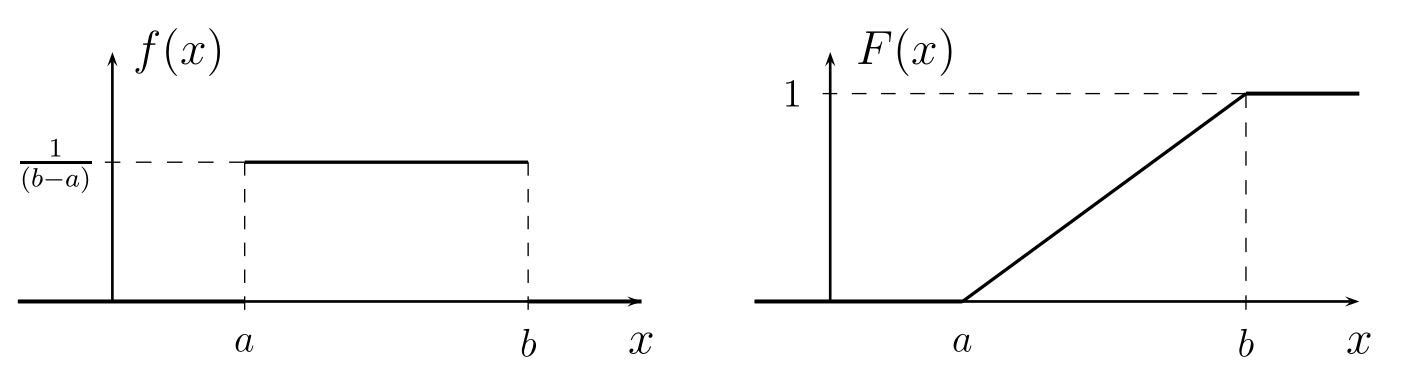
\includegraphics[width=0.5\textwidth]{img/d1.png}
    \caption{ Плотность и функция распределения $U_{a, b}$}
\end{figure}


\textbf{Показательное распределение}.
Говорят, что $\xi$ имеет показательное (экспоненциальное) распределение с параметром $\alpha > 0$ ($\xi \in \textnormal{E}_\alpha$), если $\xi$ имеет следующую плотность распределения:
\begin{equation*}
    f_\xi (x) = \left\{\begin{aligned}
        &0, &x < 0, \\
        \alpha e^{- \alpha x}, & x \geq 0.        
    \end{aligned}\right.
\end{equation*}
Функция распределения случайной величины $\xi$ непрерывна:
\begin{equation*}
    F_\xi (x) = \P (\xi < x) = \left\{\begin{aligned}
        &0, & x < 0, \\
        &1-e^{-\alpha x}, & x \geq 0.
    \end{aligned}\right.
\end{equation*}
Стоит заметить, что показательное распределение является единственным абсоютно непрерывным распределением, для которого выполнено свойство <<нестарения>> (а-ля геоетрическое):

\begin{to_thr}[]
    Пусть $\xi \in \textnormal{E}_\alpha$. Тогда для любых $x, \ y > 0$ верно, что
    $\P(\xi > x + y \mid \xi > x) = \P(\xi > y)$.
\end{to_thr}


\textbf{Нормальное распределение}. Говорят, что $\xi$ имеет \textit{нормальное} (\textit{гауссовское}) распределение с параметрами $a, \, \sigma^2$, где $a \in \mathbb{R}$, $\sigma > 0$ ($\xi \in \textnormal{N}_{a, \sigma^2}$), если $\xi$ имеет плотность распределения вида
\begin{equation}
    f_\xi (x) = \frac{1}{\sigma \sqrt{2 \pi}} \, \exp \left(
        - \frac{(x-a)^2}{2 \sigma^2}
    \right), 
    \hspace{5 mm}
    x \in \mathbb{R}. 
\end{equation}
Это действительно функция распределения, ведь вспоминая интеграл Пуассона
\begin{equation*}
    I = \int_{-\infty}^{+\infty} e^{-x^2/2} \d x = \sqrt{2 \pi},
\end{equation*}
нетрудно заменой переменных свести $\int f_\xi (x) \d x$ к $I$.

\begin{to_def}
    Нормальное распределение $\textnormal{N}_{0, 1}$ называется \textit{стандартным нормальным} распределением.
\end{to_def}

Для функции распределения нормального закона $\textnormal{N}_{a, \sigma^2}$ далее будет использоваться $\Phi_{a, \sigma^2} (x)$ для функции распределения нормального закона $N_{a, \sigma^2}$. 


% \textbf{Гамма-распределение}. Говорят, что $\xi$ имеет гамма-распределение, с параметрами $\alpha > 0$, $\lambda > 0$, 
\textbf{Распределение Коши}. Говорят, что $\xi$ имеет распределение Коши с параметрами $a \in \mathbb{R}$, $\sigma > 0$ ($\xi \in \textnormal{C}_{a, \sigma}$), если $\xi$ имеет следующую плотность распределения:
\begin{equation*}
    f_\xi (x) = \frac{1}{\pi} \frac{\sigma}{\sigma^2 + (x-a)^2}, \hspace{5 mm} \forall x \in \mathbb{R}.
\end{equation*}
Плотность распределения Коши симметрична относительно $x = a$ и похожа на нормальное, но с более толыстыми хвостами на $\pm \infty$. Функция распределения случайной величины $\xi$ с распределением Коши равна
\begin{equation*}
    F_\xi (x) = \frac{1}{2} + \frac{1}{\pi} \arctg\left(
        \frac{x-a}{\sigma}
    \right).
\end{equation*}


\red{
\textbf{Гамма-распределение}.
}

\red{
\textbf{Распределение Парето}.
}



\subsection{Свойства функций распределения}
\textbf{Общие свойства функций распределения}. Функцией распределения случайной величины $\xi$ мы назвали функцию $F_\xi (x) = \P (\xi < x)$. 

\begin{to_thr}
    Любая функция распределения обладает свойствами
    \begin{itemize}
        \item[F1)] она не убвает;
        \item[F2)] в прелелах $x \to - \infty$, и $x \to + \infty$ равна $0$ и $1$ соответственно;
        \item[F3)] она в любой точке непрерывна слева.
    \end{itemize}
\end{to_thr}


\begin{to_thr}[]
    Если функция $F \colon \mathbb{R} \mapsto [0, 1]$ удовлетворяет свойствам (F1)-(F3), то $F$ есть функция распределения некоторой случайной величины $\xi$, т.е. найдётся вероятностное пространство $\langle \Omega, \mathcal F, \P \rangle$ и случайная величина $\xi$ на нём такая, что $F(x) \equiv F_\xi (x)$. 
\end{to_thr}

\begin{to_lem}
     любой точке $x_0$ разница $F_\xi (x_0 + 0) - F_{\xi} (x_0)$ равна $\P (\xi = x_0)$:
     \begin{equation*}
          F_\xi (x_0 + 0) = F_\xi (x_0) + \P (\xi = x_0) = P (\xi \leq x_0).
      \end{equation*} 
\end{to_lem}

\begin{to_lem}
    Для любой случайной величины $\xi$
    \begin{equation*}
        \P (a \leq \xi < b) = F_\xi (b) - F_\xi (a).
    \end{equation*}
\end{to_lem}




\textbf{Функция распределения дискретного распределения}. Как мы поним, функция распределения может быть найдена по талице распределения, как сумма $F_\xi (x) = \P( \xi < x) = \sum_k \P(\xi = a_k)$, где $a_k < x$.

\begin{to_lem}
    Случайная величина $\xi$ имеет дискретное распределение тогда и только тогда, когда функция распределения $F_\xi (x)$ имеет в точках $a_i$ скачки с величиной $p_i = \P(\xi = a_i) = F_\xi (a_i +0) - F_\xi (a_i)$, и растёт только за счёт скачков.
\end{to_lem}


\textbf{Свойства абсолютно непрерывного распределения}. Пусть слу-
чайная величина $\xi$ имеет абсолюлютно непрерывное распределение с плотностью $f_\xi (t)$. Тогда функция распределения может быть найдена, как интеград. 

\begin{to_lem}
    Если случайная величина $\xi$ имеет абсолютно непрерывное распределение, то её функция распределения всюду непрерывна. Более того её функция распределенеия дифференцируема почти всюду: $f_\xi (x) = F'_\xi (x) = d_x F_\xi (x)$. 
\end{to_lem}


\red{
\textbf{Функция распределения сингулярного распределения}.
}

\red{
\textbf{Функция распределения смешанного распределения}.
}

\subsection{Свойства нормального распределения}
\begin{to_lem}
    Для любого $x \in \mathbb{R}$ справедливо соотношение:
    \begin{equation*}
        \Phi_{a, \sigma^2} (x) = \Phi_{0, 1} \left(
            \frac{x-a}{\sigma}
        \right).
    \end{equation*}
\end{to_lem}


Аналогичное утверждение для случайных величичн: если $\xi \in \textnormal{N}_{a, \sigma^2}$, то $\eta = \frac{\xi-a}{\sigma} \in \textnormal{N}_{0, 1}$. Более того, если $\xi \in \textnormal{N}_{a, \sigma^2}$, то
\begin{equation*}
    \P (x_1 < \xi < x_2) = \Phi_{a, \sigma^2} (x_2) - \Phi_{a, \sigma^2} (x_2) = \Phi_{0, 1} \left(
        \frac{x_2 - a}{\sigma}
    \right) - \Phi_{0, 1} \left(
        \frac{x_1 - a}{\sigma}
    \right).
\end{equation*}
В общем вычисления любых вероятностей для нормального распределения сводятся к вычислению $\Phi_{0, 1} (x)$, которое обладает следующими свойствами:
\begin{itemize}
    \item $\Phi_{0, 1} (0) = 0.5, \hspace{5 mm} \Phi_{0, 1} (-x) = 1 - \Phi_{0, 1} (x)$.
    \item Если $\xi \in \textnormal{N}_{0, 1}$, то для любого $x > 0$, верно что
    $
        \P (|\xi| < x) = 1 - 2 \Phi_{0, 1} (-x) = 2 \Phi_{0, 1} (x) - 1.
    $
\end{itemize}







\section{Преобразования случайных величин}

\subsection{Измеримость функций от случайных величин}
Пусть на векторном пространстве $\langle \Omega, \mathcal F, \P\rangle$ задана случайная величина $\xi$. 

\begin{to_thr}[]
    Пусть $\xi$ -- случайная величина, а $g \colon \mathbb{R} \mapsto \mathbb{R}$ -- борелевская функция, т.е. такая, что для всякого борелевского множества $B$ его прообраз $g^{-1} (B)$ есть снова борелевское множество. Тогда $g(\xi)$ -- случайная величина.
\end{to_thr}

\subsection{Распределения функций от случайных величин}
\textbf{Линейные и монотонные преобразования}.
Если с дискретными распределениями всё понятно, то с абсолютно непрерывными чуть интереснее,  о них дальше и поговорим. Пусть случайная величина $\xi$ имеет функцию распределения $F_\xi (x)$ и плотность распределения $f_\xi (x)$. Построим с помощью борелевской функции $g \colon \mathbb{R} \to \mathbb{R}$ случайную величину $\eta = g(\xi)$,и найдём плотность распределения (если она существует). 

\begin{to_thr}[]
    Пусть $\xi$ имеет функцию распределения $F_\xi (x)$ и плотность распределения $f_\xi (x)$, и постоянная $a$ отлична от нуля. Тогда случайная величина $\eta = a \xi + b$ имеет плотность распределения
    \begin{equation*}
        f_\eta (x) = \frac{1}{|a|} f_\xi \left(
            \frac{x-b}{a}
        \right).
    \end{equation*}
\end{to_thr}


\textbf{Квантильное преобразование}. Полезно уметь строить случайные величины с заданным распределением по равномерно распределенной случайной величине.

\begin{to_thr}[]
    Пусть функция распределения $F(x) = F_\xi (x)$ непрерывна. Тогда случайная величина $\eta = F(\xi)$ имеет равномерное на отрезке $[0, 1]$ распределение. 
\end{to_thr}

\begin{to_thr}[$\mathfrak{alarm}$]
    Пусть $\eta \in U_{0, 1}$, а $F$ -- произвольная функция распределения. Тогда случайная величина $\xi = F^{-1} (\eta)$ (\textbf{<<квантильное преобразование}>>  над $\eta$) имеет функцию распределения $F$. 
\end{to_thr}

\noindent
Как следствие,
для $\eta \in \textnormal{U}_{0, 1}$
,верны следующие утверждения:
\begin{equation*}
    - \frac{1}{\alpha} \ln (1 - \eta) \in \textnormal{E}_\alpha, 
    \hspace{5 mm}  
    a + \sigma \tg (\pi \eta - \pi / 2) \in \textnormal{C}_{\alpha, \sigma},
    \hspace{5 mm}
    \Phi_{0, 1}^{-1} (\eta) \in \textnormal{N}_{0, 1}.
\end{equation*}





\section{\xmark Многомерные распределения}


\subsection{Совместное распределение}
Пусть случайные величины $\xi_1, \ldots, \xi_n$ заданы на одном вероятностном пространстве $\langle \Omega, \mathcal F, \P\rangle$.

\begin{to_def}
    Функция
    \begin{equation}
        F_{\xi_1, \ldots, \xi_n} (x_1, \ldots, x_n) = \P(
            \xi_1 < x_1, \ldots, \xi_n < x_n
        )
    \end{equation}
    называется функцией распределения вектора $(\xi_1, \ldots, \xi_n)$ или функцией \textit{совместного} распределения случайных величины $\xi_1, \ldots, \xi_n$.
\end{to_def}

\subsection{Типы многомерных распределений}
Далее рассмотрим два типичных случая, когда совместное распределение либо дискретно, либо непрерывно.
\texttt{Сингулярное распределение не является редкостью: стоит выбрать отрезок на плоскости.} 

\begin{to_def}
    Случайные величины $\xi_1, \, \xi_2$ имеют \textit{дискретное} совместное распределение, если существует конечный или счётный набор пар числе $\{a_i, b_j\}$ такой, что
    \begin{equation*}
        \sum_{i=1}^{\infty} \sum_{j=1}^{\infty} \P (\xi_1 = a_i, \ \xi_2 = b_j) = 1.
    \end{equation*}
    Таблицу, на пересечении $i$-й строки и $j$-го столбца которых стоит $\P(\xi_1 = a_i, \ \xi_2 = b_j)$, называют таблицей совместного распределения случайных величин $\xi_1$ и $\xi_2$. 
\end{to_def}

\begin{to_def}
    Случайные величины $\xi_1$, $\xi_2$ имеют \textit{абсолютно непрерывное} совместное распредеение, если существует неотрицательная функция $f_{\xi_1, \xi_2} (x, y)$ такая, что для любого множества $B \in \mathfrak B (\mathbb{R}^2)$ имеет место равенство
    \begin{equation*}
         \P \left(
            (\xi_1, \xi_2) \in B
         \right) = \iint_B f_{\xi_1, \xi_2} (x, y) \d x \d y.
     \end{equation*} 
     Функция $f_{\xi_1, \xi_2} (x, y)$ называется \textit{плотностью совместного распределения} случайных величин $\xi_1$ и $\xi_2$.
\end{to_def}

Если случайные величины $\xi_1$ и $\xi_2$ имеют абсолютно непрерывное совместное распределение, то для любых $x_1$, $x_2$ имеет место равенство
\begin{equation*}
    F_{\xi_1, \xi_2} (x_1, x_2) = \P(\xi_1 < x_1, \ \xi_2 < x_2) = \int_{-\infty}^{x_1} \left(
        \int_{-\infty}^{x_2} f_{\xi_1, \xi_2} (x, y) \d y
    \right) \d x.
\end{equation*}
По функции совместного распределения его плотность находится как смешанная частная производная:
\begin{equation*}
    f_{\xi_1, \xi_2} (x, y) = \frac{\partial^2 }{\partial x \partial y} F_{\xi_1, \xi_2} (x, y)
\end{equation*}
для почти всех $(x, y)$. 

\begin{to_thr}[]
    Если случайные величины $\xi_1$ и $\xi_2$ имеютабсолютно непреывное совместное распределение с плотностью $f(x, y)$, то $\xi_1$ и $\xi_2$ в отдельности также имеют абсолютно непрерывное распределение с плотностями:
    \begin{equation*}
        f_{\xi_1} (x) = \int_{-\infty}^{+\infty} f(x, y) \d y;
        \hspace{10 mm}
        f_{\xi_2} (y) = \int_{-\infty}^{+\infty} f(x, y) \d x.
    \end{equation*}
\end{to_thr}

\subsection{Примеры многомерных распределений}
\textbf{Многомерное нормальное распределение}. Пусть $\Sigma > 0$ -- положительно определенная симметричная матрица. Говорят, что вектор $(\xi_1, \ldots, \xi_n)$ имеет многомерное нормально распределение $\textnormal{N}_{\vv{a}, \Sigma}$ с вектором средних $\vc{a}$ и матрицей ковариации $\Sigma$, если плотность совместного распределения $f_{\xi_1, \ldots, \xi_n} (x_1, \ldots, x_n)$ равна
\begin{equation*}
    f_{\xi} (\vc{x}) = \frac{1}{\sqrt{\det \Sigma} (\sqrt{2 \pi})^n}
    \exp\left(
        - \frac{1}{2} (\vc{x}-\vc{a})\T \cdot \Sigma^{-1} \cdot (\vc{x} - \vc{a})
    \right)
\end{equation*}
В частном случае, когда $\Sigma$ -- диагональная матрица с элементами $\sigma_1^2, \ldots, \sigma_n^2$ на диагонали, совместная плотность превращается в произведение плотностей нормальных величин. Вообще это равенство означает независимость величин $\xi_1, \ldots, \xi_n$.



\subsection{Независимость случайных величин}
\begin{to_def}
    Случайные величины $\xi_1, \ldots, \xi_n$ называются \textit{независимыми} (в совокупности), если \textit{для любого} набора борелевских множеств $B_1, \ldots, B_n \in \mathfrak B (\mathbb{R})$ имеет место равенство
    \begin{equation*}
         \P (\xi_1 \in B_1, \ldots, \xi_n \in B_n) 
         =
          \P (\xi_1 \in B_1) \cdot \ldots \cdot \P (\xi_n \in B_n).
     \end{equation*}  
\end{to_def}

Определение независимости можно сформулировать в терминах функций распределения. 

\begin{to_def}
    Случайные величины $\xi_1, \ldots, \xi_n$ независимы (в совокупности), если для любых $x_1,\ldots, x_n$ имеет место равенство
    \begin{equation*}
        F_{\xi_1, \ldots, \xi_n}  (x_1, \ldots, x_n) = F_{\xi_1} (x_1) \cdot \ldots \cdot F_{\xi_n} (x_n).
    \end{equation*}
\end{to_def}

\begin{to_thr}[]
    Случайные величины $\xi_1, \ldots, \xi_n$ с абсолютно непрерывными распределениями независимы (в совокупности) тогда и только тогда, когда плотность их совместного распределения существует и равна произведению плотностей, т.е.для любых $x_1, \ldots, x_n$ имеет место равенство:
    \begin{equation*}
        f_{\xi_1, \ldots, \xi_n} (x_1, \ldots, x_n) = f_{\xi_1} (x_1) \cdot \ldots \cdot f_{\xi_n} (x_n).
    \end{equation*}
\end{to_thr}

\subsection{Функции от двух случайных величин}
Пусть $\xi_1$ и $\xi_2$ -- случайные величины с плотностью совместного распределения $f_{\xi_1, \xi_2} (x_1, x_2)$, и задана борелевская функция $g \colon  \mathbb{R}^2 \mapsto \mathbb{R}$. Требуется найти функцию (и плотность, если повезет) распределения случайной величины $\eta = g(\xi_1, \xi_2)$. 

\begin{to_thr}[]
    Пусть $x \in \mathbb{R}$, и область $D_x \subseteq \mathbb{R}^2$ состоит из точек $(u, v)$ таких, что $g(u, v) < x$. Тогда случайная величина $\eta = g(\xi_1, \xi_2)$ имеет функцию распределения
    \begin{equation*}
        F_\eta (x) = \P (g(\xi_1, \xi_2) < x) = \P \left((\xi_1, \xi_2) \in D_x\right) = \iint_{D_x} f_{\xi_1, \xi_2} (u, v) \d u \d v.
    \end{equation*}
\end{to_thr}

Если $\xi_1$ и $\xi_2$ независимы, то распределение $g(\xi_1, \xi_2)$ полностью определяется частными распределениями величин $\xi_1$ и $\xi_2$.

\begin{to_thr}[формула свёртки]
    Если случайные величины $\xi_1$ и $\xi_2$ независимы и имеют абсолютно непрерывные распределения с плотностями $f_{\xi_1} (u)$ и $f_{\xi_2} (v)$, то плотность распределения суммы $\xi_1 + \xi_2$ существует и равна <<свёртке>> плотностей $f_{\xi_1}$ и $f_{\xi_2}$:
    \begin{equation}
        f_{\xi_1 + \xi_2} (t) = \int_{-\infty}^{+\infty} f_{\xi_1} (u) f_{\xi_2} (t-u) \d u =
        \int_{-\infty}^{+\infty}  f_{\xi_2} (u) f_{\xi_1} (t-u) \d u.
    \end{equation}
\end{to_thr}


\section{Числовые характеристики распределений}

\subsection{Математическое ожидание случайной величины}
Далее будет использовать термин \textit{математического ожидания}, и также можно встретить наименования: \textit{среднее значение}, \textit{первый момент}. 

\begin{to_def}
    \textit{Математическим ожиданием} 
    $\E(\xi)$ случайной величины $\xi$ с дискретным распределением называется \textit{число}
    \begin{equation*}
        \E (\xi) = \sum_k a_k p_k = \sum_k a_k \P (\xi = a_k),
    \end{equation*}
    если данный ряд абсолютно сходится, т.е. если $\sum_i |a_i| \, p_i < +\infty$. В противном случае говорят, что математическое ожидание \textit{не существует}. 
\end{to_def}


\begin{to_def}
    \textit{Математическим ожиданием} $\E (\xi)$ случайное величины $\xi$ c абсолютно непрерывным распределением с плотностью распределения $f_\xi (x)$ называется \textit{число}
    \begin{equation*}
        \E (\xi) = \int_{-\infty}^{+\infty} 
        x f_\xi (x) \d x,
    \end{equation*}
    если этот интеграл абсолютно сходится, т.е. если $\int |x| f_\xi (x) \d x < + \infty$. 
\end{to_def}



\subsection{Свойства математического ожидания}
Далее всегда предполагается, что матожидание существует. 

(E1) Для $\forall$ борелевской $g \colon  \mathbb{R} \mapsto \mathbb{R}$, для дискретного и непрерывного распределения, при существующем $\E$:
\begin{equation*}
    \E g(\xi) = \sum_k g(a_k) \P(\xi = a_k),
    \hspace{10 mm}
    \E g(\xi) = \int_{-\infty}^{+\infty} g(x) f_\xi (x) \d x.
\end{equation*}

(E3) Матожидание линейно по константам: $\E (c \xi) = c \E (\xi)$. 

(E4) Матожидание суммы \textit{любых} случайных величин равно сумме их матожиданий: $\E (\xi + \eta) = \E (\xi) + \E (\eta)$.

(E7) Если $\xi$ и $\eta$ независимы и их матожидания существуют, то $\E (\xi \eta) = \E(\xi) \cdot \E(\eta)$.













\subsection{Дисперсия и моменты старших порядков}
\begin{to_def}
    Пусть $\E |\xi|^k < + \infty$. Число $\nu_k = \E \xi^k$ называется \textit{моментом порядка $k$}, или \textit{$k$-м моментом}  случайной величины $\xi$, число $\E |\xi|^k$ называется \textit{абсолютным $k$-м моментом}. Число
    $
        \E \left[
            \xi - \E (\xi)
        \right]^k
    $
    называется \textit{центральным $k$-м моментом}, $\E |\xi - \E \xi|^2$ -- \textit{абсолютным центральным $k$-м моментом}.
\end{to_def}

\begin{to_def}
    Число $\D (\xi) = \E (\xi - \E \xi)^2$ (центральный момент второго порядка)  называется \textit{дисперсией} случайной величины $\xi$.  Другими словами, это <<среднее значение квадрата отклонения случайной величины $\xi$ от своего среднего>>.
\end{to_def}

\begin{to_def}
    Число $\sigma = \sqrt{ D \xi}$ называют \textit{среднеквадратичным отклонением} случайной величины $\xi$.
\end{to_def}

\begin{to_thr}[неравенство Йенсена]
    Пусть вещественнозначная функция $g$ выпукла. Тогда для любой случайной величины $\xi$ с конечным первым моментом верно неравенство
    \begin{equation*}
        \E g(\xi) \geq g (\E \xi),
    \end{equation*}
    где для вогнутых функций знак неравенства меняется на противоположный. 
\end{to_thr}

\begin{to_lem}
    Если $\E |\xi|^t < \infty$, то для любого $0 < s < t$ верно, что
    \begin{equation*}
        \sqrt[s]{\E |\xi|^s} \leq \sqrt[t]{\E |\xi|^t}.
    \end{equation*}
\end{to_lem}

\noindent
Также из неравенства Йенсена вытекает ряд удобных неравенств:
\begin{equation*}
    \E e^{\xi} \geq e^{\E \xi},
    \hspace{5 mm}
    \red{\ldots}
\end{equation*}

\subsection{Свойства дисперсии}
Во всех свойствах ниже предполагается существование вторых моментов случайных величин.

(D1) 
Дисперсия может быть вычислена по формуле $\D \xi = \E \xi^2 - (\E \xi)^2$.
\begin{equation*}
    \D \xi = \E (\xi - E \xi)^2 = \bigg/
        a = \E \xi
    \bigg/ = \E (\xi^2) - 2 a \E \xi + a^2 = \E \xi^2 - (\E \xi)^2.
\end{equation*}

(D2)
Считая $c$ константной: $\D (c \xi) = c^2 \D \xi$. 

(D3)
Дисперсия нетрицательна: $\D \xi \geq 0$, более того обращается в ноль, только при $\xi = \const$ почти наверное. 

(D4)
$\D (\xi + c) = \D \xi$.

(D5)
Если $\xi$ и $\eta$ независимы, то $\D (\xi + \eta) = \D \xi + \D \eta$. Вообще верна формула
\begin{equation}
    D(\xi + \eta) = \D \xi + \D \eta + 2 (\E (\xi \eta) - \E \xi \E \eta).
\end{equation}

(D6)
Минимум среднеквадратичного отклонения $\xi$ от точек числовой прямой есть $\D \xi$:
\begin{equation*}
    \D \xi = \E (\xi - \E \xi)^2 = \min_a \E (\xi - a)^2.
\end{equation*}

\subsection{Математические ожидания и дисперсии стандартных распределений}
Посчитаем несколько характерных значений для различных распределений:

\begin{table}[h]
\centering
\begin{tabular}{c|ccc}
 Имя & $\E \xi$ & $\E \xi^2$ & $\D \xi$ \\ 
 \hline
 $\textnormal{B}_{1, p}$ & $p$ & $p$ & $pq$ \\
 $\textnormal{G}_{p}$ & $1/p$ &  & $q p^{-2}$ \\
 $\Pi_{\lambda}$ & $\lambda$ & $\lambda^2 + \lambda$ & $\lambda$ \\
 $\textnormal{U}_{a, b}$ & $(a+b)/2$ & $\frac{1}{3} (a^2 + ab + b^2)$ & $\frac{1}{12} (b-a)^2$ \\
 $\textnormal{N}_{0,1}$ & $0$ & $1$ & $1$ \\
 $\textnormal{N}_{a,\sigma}$ & $a$ &  & $\sigma^2$ \\
 $\textnormal{E}_{\alpha}$ & $1!/\alpha^1$ & $2!/\alpha^2$ & $1/\alpha^2$ \\
 $\textnormal{C}_{0, 1}$ & $\nexists$  & $\nexists$  & $\nexists$ \\
\end{tabular}
\end{table}

\subsection{Другие числовые характеристики распределений}
Далее кратко познакомимся с другими показателями из статистики. 

\begin{to_def}
    \textit{Медианой} распределения случайной величины $\xi$ называется любое из чисел $\mu$ таких, что
    \begin{equation*}
        \P (\xi \leq \mu) \geq \frac{1}{2}, \hspace{5 mm}
        \P (\xi \geq \mu) \geq \frac{1}{2}.
    \end{equation*}
    Обобщая, приходим к понятию \textit{квантили} уровня $\delta \in (0, 1)$, так назывется решение уравнения $\P (x_\delta) = \delta$, где $x_\delta$ отрезает площадь $\delta$ слева от себя и $1-\delta$ справа. 
\end{to_def}

Вообще ещё есть такой зоопарк, что квантили уровней кратных $0.01$ в прикладной статистике называют \textit{процентилями}, кратных $0.1$ -- \textit{децилями}, кратных $0.25$  -- \textit{квартилями}.

\begin{to_def}
    \textit{Модой} абсолютно непрерывного распределения называют любую точку локального максимума плотности распределения. Для дискретных распределений модой считают любое значение $a_i$, вероятность которого больше соседних.
\end{to_def}

Для описания \textit{унимодеальных} распределений используют следующие величины:

\begin{to_def}
    \textit{Коэффициентом асимметрии} распределения с конечным третьим моментом называют число
    \begin{equation*}
        \beta_1 = \E \left(
            \frac{x-a}{\sigma}
        \right)^3,
    \end{equation*}
    где $a = \E \xi$,  а $\sigma = \sqrt{D \xi}$. 
\end{to_def}

Для симметричных распределений коэффициент асимметрии равен нулю, если $\beta_1 > 0$, то график плотности имеет более крутой наклон слева, и более пологий справа. 

\begin{to_def}
    \textit{Коэффициентом эксцесса} распределения с конечным четвертым моментом называется число
    \begin{equation*}
        \beta_2 = \E \left(
            \frac{\xi - a}{\sigma}
        \right) - 3,
    \end{equation*}
    где $a = \E \xi$,  а $\sigma = \sqrt{D \xi}$. 
\end{to_def}

Для нормального распределения $\beta_2 = 0$, при $\beta_2 > 0$ плотность распределения имеет более острую вершину, чем у нормального распределения. 




\subsection{Производящие функции}
Дискретные величины, рассмотренные раннее, принимают только целые значения $X = 0, 1, \ldots$. Нахождение числовых характеристик упрощается, если рассматреть \textit{производящие функции}.

\begin{to_def}
    \textit{Производящей функцией} дискретной целочисленной случайной величины $\xi$ с законом распределения
    $\P (\xi = k) = p_k$ , где $k = 0, 1, \ldots$ называется функция, заданная степенным рядом
    \begin{equation}
        \E(s^\xi) = P (s) = p_0 + p_1 s + p_2 s^2 + \ldots,
    \end{equation}
    который сходится по крайней мере для $|s| \leq 1$. 
\end{to_def}

\begin{to_thr}[]
    Производящая функция суммы независимых случайных величин $\xi$ и $\eta$ равна произведению производящих функций слагаемых
    \begin{equation}
        P_{\xi + \eta} (s) = P_\xi (s) \cdot P_\eta (s).
    \end{equation}
\end{to_thr}

Так например для биномального распределения производящая функция примет вид
\begin{equation*}
    P (s) = (q + ps)^n.
\end{equation*}
А для геометрического закона распределения
\begin{equation*}
    \P (s) = p s + p q s^2 + p q^2 s^3 + \ldots = \frac{ps}{1-qs}.
\end{equation*}
В случае же Пуассона
\begin{equation*}
    P (s) = \sum_{k=0}^{\infty} \frac{\lambda^k}{k!}e^{-\lambda} s^k = e^{-\lambda} \sum_{k=0}^\infty 
    \frac{(\lambda s)^k}{k!} = e^{-\lambda} e^{\lambda s} = e^{\lambda (s-1)}.
\end{equation*}

\begin{to_thr}
    Сумма независимых случайных величин, распределенных по закону Пуассона, распределена по тому же закону.
\end{to_thr}

\begin{to_thr}[]
    Для дискретной случайной величины $\xi$ с производящей функцией $\P (s)$ выполняются следующие требования:
    \begin{equation}
        \E (\xi) = P'_s (1),
        \hspace{10 mm}
        \D (\xi) = P''_{s,s} (1) + P'_s (1) - [P'_{s} (1)]^2.
    \end{equation}
\end{to_thr}




% \subsection{Числовые характеристика случайного вектора}
% \begin{to_thr}[]
    Для матожидания функции $\varphi(x, y)$ от компонент случайного вектора $(\xi, \eta)$ справедлива формула
    \begin{equation*}
        \E \varphi(\xi, \eta) = 
        \int_{-\infty}^{+\infty} \int_{-\infty}^{+\infty} \varphi(\xi, \eta) 
        f_{\xi, \eta} (x, y) \d x \d y.
    \end{equation*}
\end{to_thr}

\begin{to_def}
    \textit{Начальным моментом порядка} $(k, l)$ называется математическое ожидание функции $x^k y^l$:
    \begin{equation*}
        \nu_{k, l} = \E (\xi^k \eta^l)
        =
        \int_{-\infty}^{+\infty} \int_{-\infty}^{+\infty} 
        x^k y^l f_{\xi, \eta} (x, y) \d x \d y.
        .
    \end{equation*}
\end{to_def}


\red{
\begin{to_def}
    \textit{Центральным моментом порядка} $(k, l)$
    называется математическое ожидание функции $(\xi - \E \xi)^k (\eta - \E \eta)^l$:
    \begin{equation*}
        \mu_{k, l} \overset{\mathrm{def}}{=}  \E \left(
            (\xi - \E \xi)^k (\eta - \E \eta)^l
        \right) 
        =
        \int_{-\infty}^{+\infty} 
        \int_{-\infty}^{+\infty} 
        (x - \E \xi)^k (y - \E \eta)^l f_{\xi, \eta} (x, y) \d x \d y.
    \end{equation*}
\end{to_def}
}


\begin{to_def}
    Для набора случайных величин $\xi_1, \ldots, \xi_n$ \textit{ковариационной матрицей} $C = (c_{ij})$ и \textit{корреляционной матрицей} $\R = (\rho_{ij})$ называют матрицы порядка $n$, состоавленные из всех парных ковариаций, и всех парны коэффициентов корреляции
    \begin{equation*}
        c_{ij} = \cov (\xi_i,\, \xi_j),
        \hspace{10 mm}
        \rho_{ij} = \rho(\xi_i,\, \xi_j).
    \end{equation*}
\end{to_def}
 
 Стоит заметить, что эти матрицы симметричны, неотрицательно определены, а также неотрицательны их определители, более того $\det R \leq 1$.

\subsection{Вычисление моментов через производящие функции}
\begin{to_def}
    \textit{Производящей функцией моментов} случайной величины $\xi$ называют математическое ожидание случайной величины $e^{s \xi}$, где $s$ -- действительный параметр:
    \begin{equation}
        \psi_\xi (s) = \E (e^{s \xi}).
    \end{equation}
\end{to_def}

\begin{to_thr}[]
    Если случайная величина $\xi$ имеет начальный момент порядка $n$, то производящая функция $\psi_\xi (s)$ $n$ раз дифференцируема по $s$, и для всех $k \leq n$ выполняется соотношение
    \begin{equation}
        \nu_k = \psi^{(k)}_\xi (0).
    \end{equation}
\end{to_thr}

Действительно, разлагая функции моментов в ряд Маклорена, можно получить её разложение в ряд с начальными моментами
\begin{equation*}
    \psi_\xi (s) = 1 + \nu_1 s + \frac{\nu_2}{2!} s^2 + \ldots
\end{equation*}



\section{Числовые характеристики зависимости}

\subsection{Ковариация двух случайных величин}
Дисперсия суммы двух случайных величин равна
\begin{equation*}
    \D (\xi + \eta) = \D \xi + \D \eta + 2 \left(\E(\xi \eta) - \E (\xi) \E (\eta)\right).
\end{equation*}
Величина $\E (\xi \eta) - \E \xi \E \eta = 0$, если $\xi$ и $\eta$ независимы, но это верно только в одну сторону, поэтому эту величину используют как <<индикатор наличия зависимости>> между двумя случайными величинами. 

\begin{to_def}
    \textit{Ковариацией} $\cov(\xi, \eta)$ случайных величин $\xi$ и $\eta$ называется число
    \begin{equation}
        \cov (\xi, \eta) = \E \big[(\xi-\E \xi)(\eta - \E \eta)\big].
    \end{equation}
\end{to_def} 

\noindent
Для ковариации справедливы следующие равенства:
\begin{equation*}
    \cov(\xi ,\eta) = \E (\xi \eta) - \E (\xi) \E (\eta);
    \hspace{5 mm}
    \cov (\xi, \xi) = \D (\xi);
    \hspace{5 mm}   
    \cov(\xi, \eta) = \cov(\eta, \xi);
    \hspace{5 mm}
    \cov (c \xi, \eta) = c \, \cov (\xi, \eta).
\end{equation*}

\begin{to_lem}
    Дисперсия суммы нескольких случайных величин вычисляется по формуле:
    \begin{equation}
        \D (\xi_1 + \ldots + \xi_n) = 
        \sum_{i=1}^{n} \D (\xi_i) + \sum_{i \neq j} \cov (\xi_i, \xi_j) 
        =
        \sum_{i, j} \cov(\xi_i, \xi_j).
    \end{equation}
\end{to_lem}

Если ковариация $\cov (\xi, \eta) \neq 0$, то $\xi$ и $\eta$ зависимы. Найти совместное распределение бывает сложнее, чем посчитать $\E (\xi \eta)$, поэтому, если повезет, и $\E (\xi \eta) \neq \E (\xi) \E (\eta)$, то, не находя совместное распределение, мы обнаружим зависимость $\xi$ и $\eta$, не находя их совсметного распределения.
\texttt{Это очень хорошо.} 

Однако есть проблема -- ковариация не безразмерно, поэтому большие значения ковариции не говорят о более сильной зависимости. Хотелось бы как-то отнормировать $\cov (\xi, \eta)$, получив <<безразмерную>> величину. Так мы приходим к коэффициенту корреляции. 



\subsection{Коэффициент корреляции}
\begin{to_def}
    \textit{Коэффициентом корреляции} $\rho (\xi, \eta)$ случайных величин $\xi$ и $\eta$, дисперсии которых существуют и отличны от нуля, называется число
    \begin{equation}
        \rho (\xi, \eta) = 
        \frac{\cov (\xi, \eta)}{\sqrt{\D \xi} \sqrt{\D \eta}}.
    \end{equation}
\end{to_def}

Можно наполнить это достаточно глубоким смыслом. На самом деле это <<косинус угла>> между двумя элементами $\xi - \E \xi$ и $\eta - \E \eta$ гильбертова пространства, образованного случайными величинами с нулевым матожиданием и конечным вторым моментом. Пространство набжено скалярным произведением $\cov (\xi, \eta)$ и <<нормой>>, равной корню из дисперсии, или $\sqrt{ \cov (\xi, \xi)}$.

\begin{to_thr}[]
    Коэффициент корреляции обладает свойствами:
    \begin{itemize}
        \item[1)] если $\xi$ и $\eta$ независимы, то $\rho(\xi, \eta) = 0$;
        \item[2)] всегда $|\rho(\xi, \eta)| \leq 1$;
        \item[3)] $|\rho(\xi, \eta)|=1$ тогда и только тогда, когда $\xi$ и $\eta$ почти наверное линейно связаны. 
    \end{itemize}
\end{to_thr}

\begin{to_def}
    \textit{Стандартизацией} случайной величины называется преобразование
    \begin{equation}
        \hat{\xi} = \frac{\xi - \E(\xi)}{\sqrt{\D (\xi)}}.
    \end{equation}
\end{to_def}

В терминах стандартизации чуть проще записывается коэффициент корреляции:
\begin{equation*}
    \rho (\xi, \eta) = \E \left(
        \hat{\xi} \cdot \hat{\eta}
    \right).
\end{equation*}

\begin{to_def}
    Говорят, что $\xi$ и $\eta$ \textit{отрицательно коррелированы}, если $\rho(\xi, \eta) < 0$; \textit{положительно коррелированы}, если $\rho (\xi, \eta) > 0$; \textit{некоррелированы}, если $\rho(\xi, \eta) = 0$. 
\end{to_def}

\begin{to_lem}
    Для любых случайных величин $\xi$ и $\eta$ с конечной и ненулевой дсперсией при любых постоянных $a \neq 0$ и $b$ имеет место равенство
    \begin{equation}
        \rho (\alpha \xi + b, \eta) = \sign(a) \cdot \rho (\xi, \eta).
    \end{equation}
\end{to_lem}


\noindent
\red{Разобрать пример 67 и далее.}




\section{Характеристические функции}

\subsection{Определение и примеры}
\begin{to_def}
    Функция $\varphi_\xi (t) = \E \left(
        e^{i t \xi}
    \right)$ вещественной переменной $t$ называется \textit{характеричтической функцией} случайной величины $\xi$.
\end{to_def}

Например, если характеристическая функция имеет стандратное нормальное распределение, то её характеристическая функция равна
\begin{equation*}
    \varphi_\xi (t) = \frac{1}{\sqrt{2\pi}} \int_{-\infty}^{+\infty} e^{i t x} e^{- x^2/2} \d x = 
    \frac{1}{\sqrt{2 \pi}} \int_{-\infty}^{+\infty} =
    \frac{e^{-t^2/2}}{\sqrt{2 \pi}} \int_{-\infty}^{+\infty} e^{- (x-it)^2/2} \d (x-it) = e^{-t^2/2}.
\end{equation*}


\subsection{Свойства характеристических функций}
(Ф1). Характеристическая функция всегда существует: $|\varphi_\xi (t) | = |\E e^{i t \xi} | \leq 1$.

(Ф2). По харакетристической функции однозначно восстанавливается распределение. Например, если модуль характеристической функции интегрируем на всей прямой, то 
\begin{equation*}
    f_\xi (x) = \frac{1}{2\pi} \int_{-\infty}^{+\infty} e^{-itx} \varphi_x (t) \d t.
\end{equation*}

(Ф3). Характерестическая функция случайной величины $a + b \xi$ связана с характеристической функцией случайной величины $\xi$ равенством
\begin{equation*}
    \varphi_{a + b \xi} (t) = \E e^{i t (a + b \xi)} = e^{i t a} \E \left(
        i (tb) \xi
    \right) = e^{i t a} \varphi_\xi (tb).
\end{equation*}

(Ф4). Характеристическая функция суммы независимых случайных величин равна произведению характеричтических функций слагаемых: если случайные величины $\xi$ и $\eta$ независимы, то
\begin{equation*}
    \varphi_{\xi + \eta} (t) = \E e^{i t (\xi + \eta)} = \E (e^{i t \xi}) \E (e^{i t \eta}) = \varphi_\xi (t) \varphi_\eta (t).
\end{equation*}
\texttt{Собственно, это очень простой и приятный инструмент для доказательства \textit{устойчивости} распределений}. \red{Чем надо было бы и воспользоваться}.

(Ф5). Пусть существует момент порядка $k \in \mathbb{N}$ случайной величины $\xi$. Тогда характеристическая функция $\varphi_\xi (t)$ непрерывно дифференцируема $k$ раз и её $k$-я производная в \textit{нуле} связана с моментом порядка $k$ равенством
\begin{equation*}
    \varphi_\xi^{(k)} (0) = \left(
        \frac{d^k }{d t^k} \E e^{i t \xi}
    \right) \bigg|_{t=0} = \left(
        \E i^k \xi^k e^{i t \xi}
    \right) \bigg|_{t=0} = i^k \E(\xi^k).
\end{equation*} 

\begin{to_lem}
    Для случайной величины $\xi$ со стандартным нормальным распределением момент чёного порядка $2k$ равен
    \begin{equation*}
        \E (\xi^{2k}) = (2 k - 1) !! = (2k -1) \cdot (2k-3) \cdot \ldots \cdot 3 \cdot 1.
    \end{equation*}
    Все моменты нечётных порядков существуют и равны нулю.
\end{to_lem}

\texttt{Как только появились производные высших порядков, самое время разложить функцию в ряд Тейлора:} 

(Ф6). Пусть существует момент порядка $k \in \mathbb{N}$ случайной величина $\xi$, тогда характеричтическая функция $\varphi_\xi (t)$ в окрестности точки $t = 0$ разлагается в ряд Тейлора
\begin{equation*}
    \varphi_\xi (t) = \varphi_\xi (0) + \sum_{j=1}^{k} \frac{t^j}{j!} \varphi_\xi^{(j)} (0) + o(|t^k|) 
    = 
    1 + \sum_{j=1}^{k} \frac{i^j t^j}{j!} \E (\xi^j) + o(|t^k|).
\end{equation*}

\begin{to_thr}[теорема о непрерывно соответствии]
    Случайные величины $\xi_n$ слабо сходятся к случайной величине $\xi$ тогда и только тогда, когда для любого $t$ характеристические функции $\varphi_{\xi-b} (t)$ сходятся к  характеристической функции $\varphi_\xi (t)$. 
\end{to_thr}



\section{Сходимость последовательностей случайных величин}

\subsection{Определение и примеры}
Плотность многомерного нормального распределения:
\begin{equation*}
    f_\xi (\vc{x}) = \left[
        (\sqrt{2\pi})^n \sqrt{\det \Sigma}
    \right]^{-1} \cdot \exp\left(
        - \frac{1}{2} (\vc{x}-\vc{\mu})\T \Sigma^{-1} (\vc{x} - \vc{\mu})
    \right),
\end{equation*}
где $\Sigma$ -- симметричная, положитеьно определенная матрица. 




% Прямо сейчас работает всё работает convert.
% Хочется научить onvert правильно оценивать результаты скиллов.
% Есть кучка диалогов -- неразмеченны. 

% Реальное качество -- frontend -- максимум. 
% Добавить кнопку -- проблема в диалоге. 


% пнуть федора про сайт
% доучить convert на наших данных
% у конверт проблема -- все ответы (я не знаю, я не понял, не уверен) -- проблема
% 
% 
